\begin{itemize}
\item \textbf{Complexity analysis}
\item general idea: translate classical planning -> language-recognition problem and examine its complexity
\item Language L, alphabet A
\item recognition procedure R(x): yes iff $x \in L$, else no or fail to terminate

	\begin{itemize}
	\item \textbf{Plan-Existence} P
	\item Problem has solution
	\item \textbf{Plan-Length} (P,n)
	\item Problem has solution <= n
	\end{itemize}

\item Runtime, space complexity

\item \textbf{Restrictions of classical planning}
\begin{itemize}
	\item Operators are fixed or input?
	\item Allow infinite initial states?*	
	\item Allow function symbols?*
	\item Allow negative effects?
	\item Allow neg. preconditions?
	\item Allow >1 preconditions?
	\item Operators have conditional effects?*
\end{itemize}

\item *: outside CP

\item \textbf{(Un)decidability}

\begin{tabular}{|c|c|c|}
\hline 
& \multicolumn{2}{c|}{Decidability} \\ 
\hline 
function symbols & Plan-Existence &Plan-Length \\ 
\hline 
no (CP) & dec & dec \\ 
\hline 
yes & semidec & dec \\ 
\hline 
\end{tabular} 


\item \textbf{Complexity results}
\item Well I guess, Plan-Existence is less complex than Plan-Length (AM?)

\item \textbf{Equivalences}
\item Set-theoretic and classical are basically identical
\item Both: exponential blowup (input)
\item Class. and state-var are basically equivalent 
\item (state-var:some restrictions not possible)

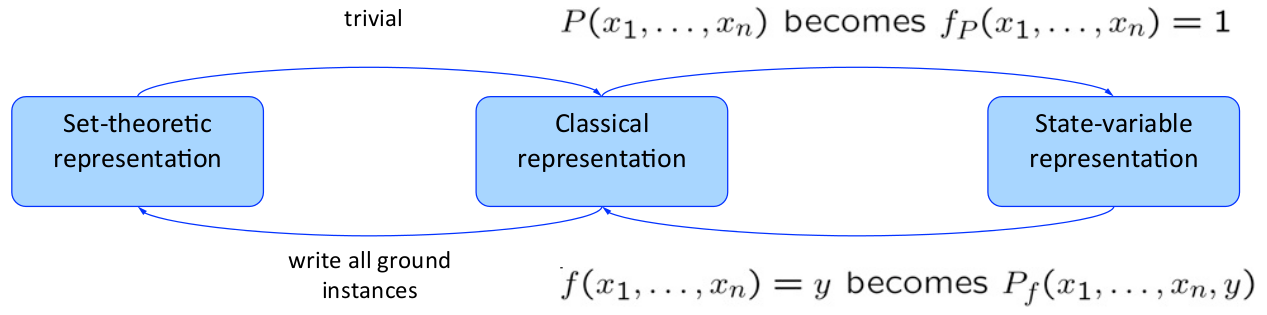
\includegraphics[width=0.48\textwidth]{./img/conversions.png}

\end{itemize}